\section{Platinum---Spin Hall conductivity}
\label{sec29:PtSHC}

\begin{itemize}
	\item Outline: {\it Calculate spin Hall conductivity (SHC) and 
			plot Berry curvature-like term  
			of fcc Pt considering spin-orbit coupling. 
			To gain a better understanding of this example, 
			it is suggested to read Ref.~\onlinecite{qiao-prb2018} for a detailed 
			description of the theory and Ch.~12.5 of the User Guide.}
\end{itemize}

\begin{itemize}
	\item[1-6] {\it Compute the MLWFs, spin Hall conductivity and 
		{\tt kpath}, {\tt kslice} plots.} 
\end{itemize}

\subsection*{Spin Hall conductivity}

\begin{itemize}
	\item {\it SHC converges rather slowly with k-point sampling, and a $25 \times 25 \times 25$ kmesh does not yield a well-converged value.
	To get a converged SHC value, increase the density of kmesh and 
	then compare the converged result with those obtained in 
	Refs.~\onlinecite{qiao-prb2018} and \onlinecite{guo-prl2008}.}

	The file {\tt Pt-shc-fermiscan.dat} contains the calculated SHC. 
	The SHC for a $25\times25\times25$ kmesh are shown in the snippet below. 
	 
\begin{tcolorbox}[title=$25\times25\times25$ kmesh,sharp corners,boxrule=0.5pt]
{\small
\begin{verbatim}
#No.   Fermi energy(eV)   SHC((hbar/e)*S/cm)
   1     6.000000    0.00000000E+00
...
 120    17.900000    0.17230482E+04
 121    18.000000    0.17054542E+04
...
 201    26.000000    0.22665760E+03
\end{verbatim}
}
\end{tcolorbox}

The calculated Fermi energy obtained from {\tt Quantum ESPRESSO} is $17.9919$ eV. 
It may vary among different calculations due to the differences between versions of {\tt Quantum ESPRESSO} or compilers, 
and these may lead to deviations from the following results. 
However, the difference should be acceptable and the calculated SHC should be essentially the same. 

The SHC at the Fermi energy is 1705 $(\hbar/e)\mathrm{S/cm}$. 
The converged results reported in Refs.~\onlinecite{qiao-prb2018} 
and \onlinecite{guo-prl2008} are around 2200 $(\hbar/e)\mathrm{S/cm}$. 
Hence, a $25\times25\times25$ kmesh clearly gives an inaccurate value ($\sim 22.5\%$ error).

Since these are quite demanding calculations, we only report the 
value of the SHC for a $100\times100\times100$ kmesh (see snippet below). 
The value for the SHC at Fermi energy is 2207 $(\hbar/e)\mathrm{S/cm}$, which is 
in much closer agreement with the converged result from 
Refs.~\onlinecite{qiao-prb2018} and \onlinecite{guo-prl2008}.

\begin{tcolorbox}[title=$100\times100\times100$ kmesh,sharp corners,boxrule=0.5pt]
{\small
\begin{verbatim}
#No.   Fermi energy(eV)   SHC((hbar/e)*S/cm)
   1     6.000000    0.00000000E+00
...
 120    17.900000    0.21899191E+04
 121    18.000000    0.22066678E+04
...
 201    26.000000    0.24919920E+03
\end{verbatim}
}
\end{tcolorbox}

\item To complete the previous discussions, we also 
compare the Fermi energy scan plots of the two calculations as 
shown in the \Fig{fig29.3}. 
\begin{figure}[!htb]
\centering
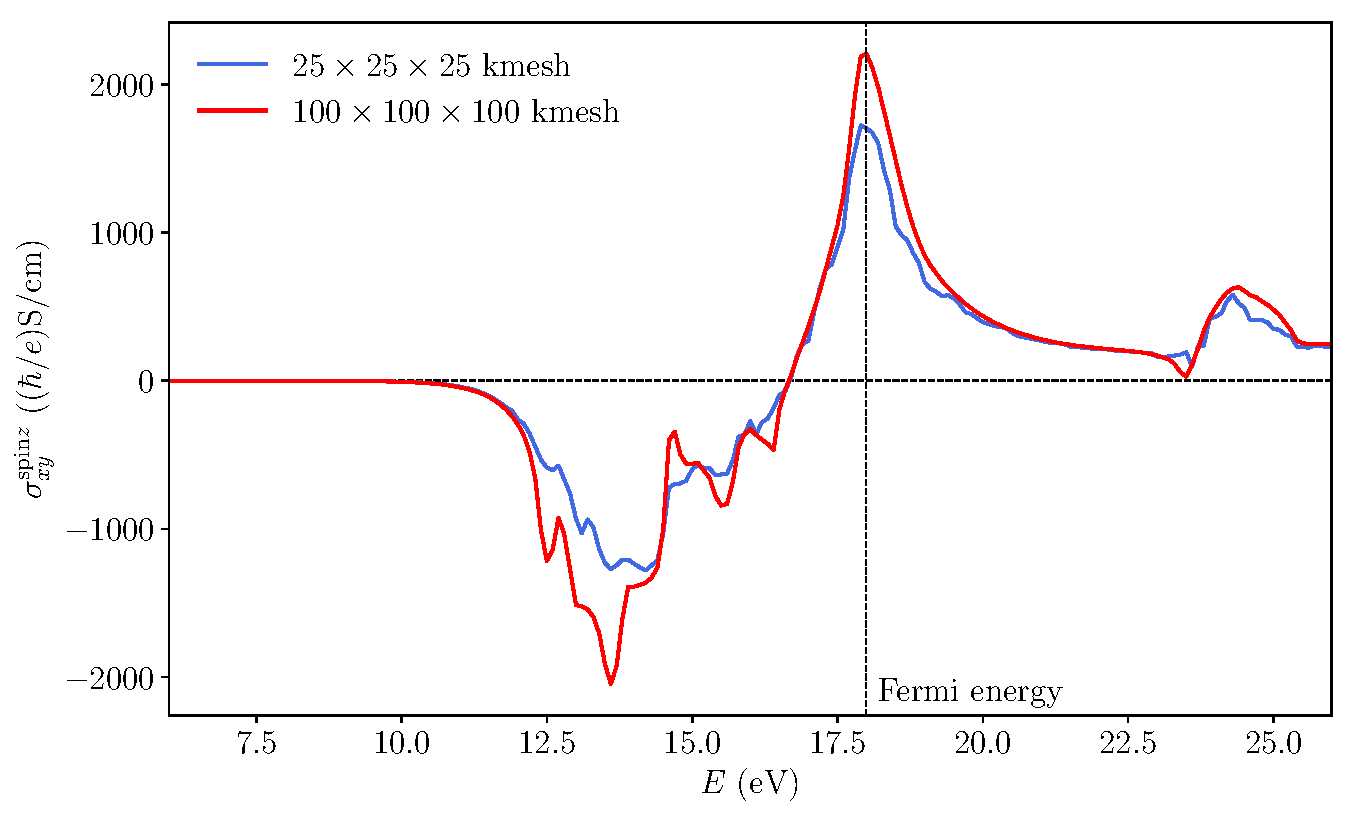
\includegraphics[width=.8\columnwidth]{figure/example29/pt_shc_kmesh.pdf}
\caption{Fermi energy scan plots for calculations 
	with $25\times25\times25$ kmesh and $100\times100\times100$ kmesh.}
\label{fig29.3}
\end{figure}

\item The {\tt seedname.wpout} will print the percentage of $k$-points which 
have been calculated at the moment, as well as the corresponding calculation time, as 
shown in the following snippet. 

\begin{tcolorbox}[title=Pt.wpout,sharp corners,boxrule=0.5pt]
{\small
\begin{verbatim}
 Properties calculated in module  b e r r y
 ------------------------------------------

   * Spin Hall Conductivity

     Fermi energy scan
 
 Calculation started
 -------------------------------
   k-points       wall      diff
  calculated      time      time
  ----------      ----      ----
       0%          0.0       0.0
      10%         22.7      22.7
      20%         36.5      13.8
      30%         50.4      14.0
      40%         64.4      14.0
      50%         78.4      14.0
      60%         92.5      14.1
      70%        106.5      14.0
      80%        120.4      13.9
      90%        134.2      13.8
     100%        147.9      13.7


 Interpolation grid: 25 25 25

 Using adaptive smearing
       adptive smearing prefactor    1.414
       adptive smearing max width    1.000 eV
       
\end{verbatim}
}
\end{tcolorbox}
This might be helpful as you can roughly 
estimate the total computational time 
of your calculation, or it might give credence to the code that it is actually functioning :). 
Note this report is merely based on the ``root'' computation node. It is accurate if the {\tt postw90} is run in serial, or the load on each node is balanced if running in parallel. However, the estimation is rough if loads are not balanced among nodes. This may happen if the performance of nodes in your cluster are not identical, or adaptive kmesh refinements are triggered so some nodes may compute much more $k$-points than others. 
Besides, if you are careful enough, you may find the diff time of 10\% is much larger than later ones. This 
is caused by some done-once-and-for-all computations carried out at the beginning, thus 
later computations are much faster. 
\end{itemize}

%\clearpage
\subsection*{Berry curvature-like term plots}
\begin{itemize}
	\item {\it The band-projected Berry curvature-like term $\Omega_{n,\alpha\beta}^{\text{spin} \gamma}({\bm k})$ 
		is defined as Eq.~(12.22) in the User Guide.}
	{\it Plot the band structure of Pt and color it 
		by the magnitude of its band-projected Berry curvature-like term $\Omega_{n,xy}^{\text{spin}z}(\bm k)$, 
		and plot the k-resolved Berry curvature-like term $\Omega_{xy}^{\text{spin}z}(\bm k)$ along the 
		same path in the BZ. }
	
	With Fermi energy set as 17.9919 eV we obtain the energy bands colored by the 
	$\Omega_{n,\alpha\beta}^{\text{spin} \gamma}({\bm k})$ 
	and the $k$-resolved Berry curvature-like term 
	$\Omega_{xy}^{\text{spin}z}(\bm k)$ along high-symmetry lines 
	as shown in \Fig{fig29.1}, which contains two plots calculated with 
	different fixed smearing width.
\end{itemize}

\begin{figure}[htb!]
	\centering
	\subfloat[With fixed smearing width of 1 eV]{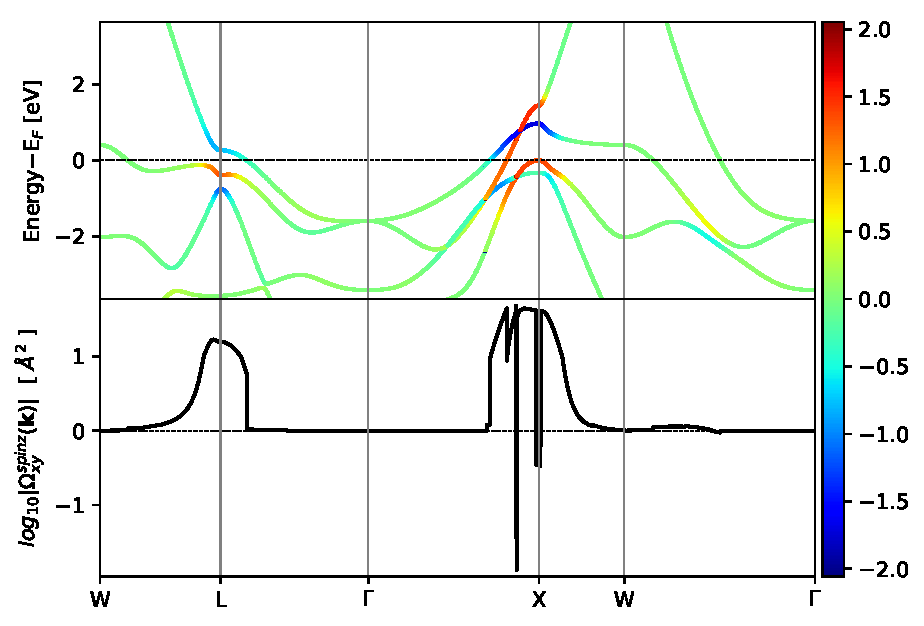
\includegraphics[width=0.45\columnwidth]{figure/example29/Pt-bands+shc_1.pdf}}\qquad
	\subfloat[With fixed smearing width of 0.05 eV]{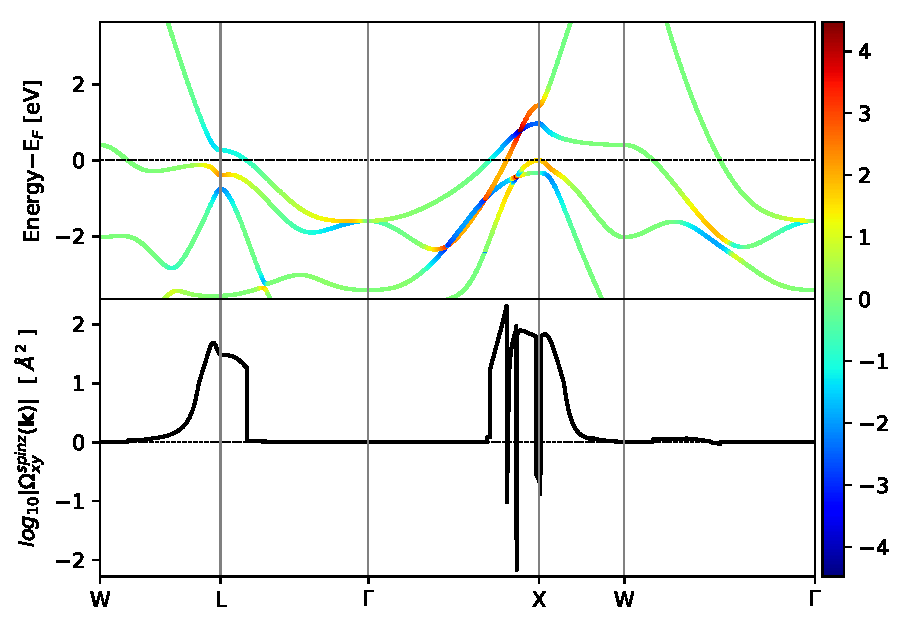
\includegraphics[width=0.45\columnwidth]{figure/example29/Pt-bands+shc_0_05.pdf}}
	\caption{Top panels: Band structure of Pt along symmetry lines W-L-$\Gamma$-X-W-$\Gamma$, colored by
		the $\Omega_{n,xy}^{\text{spin}z}({\bm k})$. 
		Bottom panels: $k$-resolved Berry curvature-like term $\Omega_{xy}^{\text{spin}z}(\bm k)$ along the symmetry lines.}
	\label{fig29.1}
\end{figure}
%\clearpage

\begin{itemize}
	\item {\it Combine the plot of the Fermi lines on the $(k_x,k_y)$ plane with a heatmap plot of the Berry curvature-like term of spin Hall conductivity.}
	
	The plots of the Fermi lines with a heatmap of $\Omega_{xy}^{\text{spin}z}(k_x,k_y,0)$ are shown in \Fig{fig29.2}.
\end{itemize}

\begin{figure}[htb!]
	\centering
	\subfloat[With fixed smearing width of 1 eV]{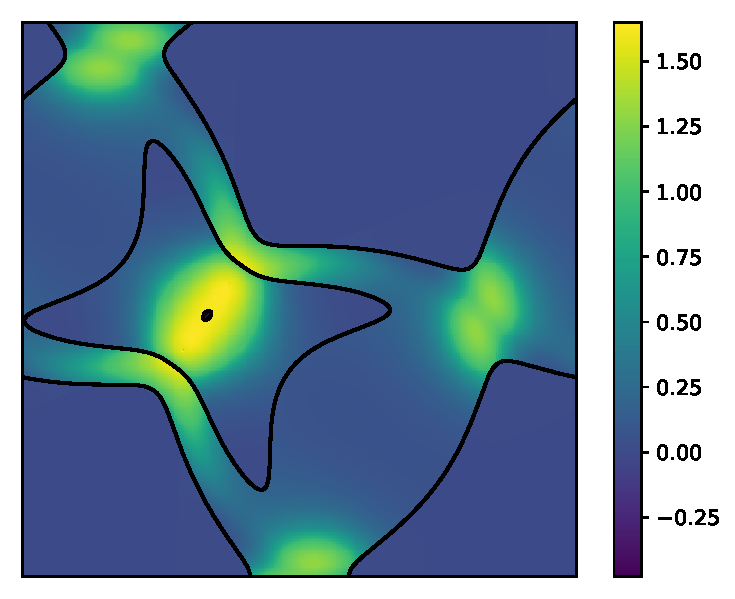
\includegraphics[width=0.45\columnwidth]{figure/example29/Pt-kslice-shc_1.pdf}}\qquad
	\subfloat[With fixed smearing width of 0.05 eV]{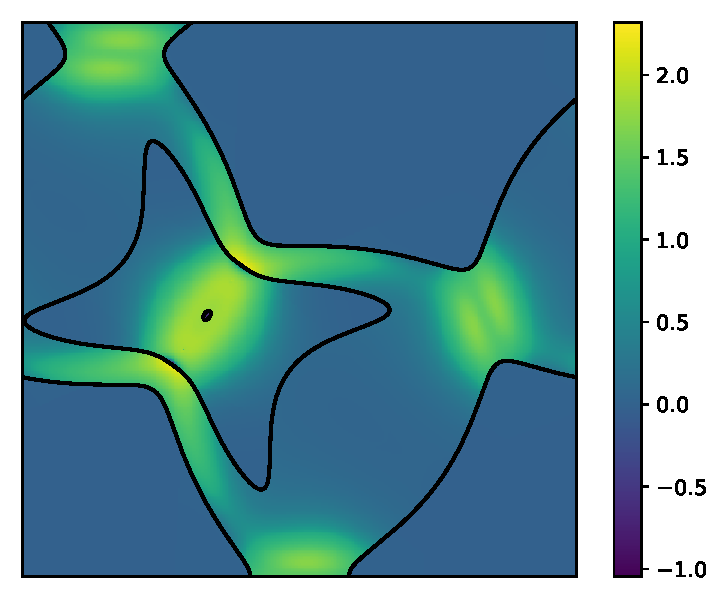
\includegraphics[width=0.45\columnwidth]{figure/example29/Pt-kslice-shc_0_05.pdf}}
	\caption{Calculated $k$-resolved Berry curvature-like term 
		$\Omega_{xy}^{\text{spin}z}(\bm k)$ in the plane $k_z=0$ 
		(note the magnitude of $\Omega_{xy}^{\text{spin}z}(\bm k)$ is in log scale). 
		Intersections of the Fermi surface
		with this plane are shown as black lines.}
	\label{fig29.2}
\end{figure}


